% ########################################################################################################################################
%
% This is the main latex file. Here we call for inputs from other files. We also define some of the main characteristics of the document.
%
% ########################################################################################################################################
%
% You likely only need to modify the "Main_Content__Write_your_essay_here.tex" file.
%
% ########################################################################################################################################

\documentclass[12pt,a4paper,oneside]{paper}
% Encoding and Language
\usepackage[utf8x]{inputenc}
\usepackage{csquotes}
\usepackage[main=english,portuguese]{babel}
\usepackage{iflang}
\usepackage{ragged2e}
\usepackage{makeidx}
\usepackage{multicol}
\usepackage[export]{adjustbox}
\usepackage{tikz-dependency}
\usepackage{fancyhdr}

% Font Configurations
\renewcommand{\rmdefault}{phv}
\renewcommand{\sfdefault}{phv}
\def\FontLn{% 16 pt normal
  \usefont{T1}{phv}{m}{n}\fontsize{16pt}{16pt}\selectfont}
\def\FontLb{% 16 pt bold
  \usefont{T1}{phv}{b}{n}\fontsize{16pt}{16pt}\selectfont}
\def\FontMn{% 14 pt normal
  \usefont{T1}{phv}{m}{n}\fontsize{14pt}{14pt}\selectfont}
\def\FontMb{% 14 pt bold
  \usefont{T1}{phv}{b}{n}\fontsize{14pt}{14pt}\selectfont}
\def\FontSn{% 12 pt normal
  \usefont{T1}{phv}{m}{n}\fontsize{12pt}{12pt}\selectfont}

% Font Encoding
\usepackage[T1]{fontenc}

% Page Geometry
\usepackage{geometry}	
\geometry{verbose,tmargin=2.cm,bmargin=2.cm,lmargin=2.cm,rmargin=2cm}

% Line Spacing
\usepackage{setspace}
\renewcommand{\baselinestretch}{1.25}

% Graphics and Figures
\usepackage{graphicx}
\usepackage{subfigure}
\usepackage{subfigmat}
\usepackage{float}

% Mathematics and Theorems
\usepackage{amsmath}
\usepackage{amsthm}
\usepackage{amsfonts}
\usepackage{dcolumn}
\usepackage{indentfirst}

% Comments and Verbatim
\usepackage{verbatim}

% Hyperlinks
\usepackage[pdftex]{hyperref}
\hypersetup{
    colorlinks,
    linkcolor=blue,
    anchorcolor=black,
    citecolor=cyan,
    filecolor=black,
    menucolor=black,
    urlcolor=teal,
    bookmarksopen=true,
    bookmarksnumbered=true
}

% Captions and References
\usepackage[figure,table]{hypcap}
\usepackage[format=plain]{caption}
\DeclareCaptionFont{georgia}{\small\fontseries{n}\fontfamily{georgia}\selectfont}
\captionsetup{labelfont=georgia,font=georgia}

% Bibliography
\usepackage[backend=biber,style=apa]{biblatex}

% Acronyms
\usepackage[printonlyused]{acronym}

% Lipsum (for placeholder text)
\usepackage{lipsum}

% Cleveref (for clever references)
\usepackage[\IfLanguageName{english}{english}{portuguese}]{cleveref}

% Colors
\usepackage{xcolor}
\usepackage{color}

% Custom Commands
\newcommand{\gray}[1]{\textcolor{gray}{#1}}

% Equation Numbering
\renewcommand{\theequation}{{\fontseries{n}\fontfamily{georgia}\selectfont\arabic{equation}}}

% Section and Subsection Fonts
\sectionfont{\Large\bfseries\fontfamily{lmss}\selectfont}
\subsectionfont{\large\bfseries\fontfamily{lmss}\selectfont}

\makeindex

\addbibresource{bibliography.bib}
\begin{document}
\pagestyle{fancy}
\fancyhf{} % Clear previous settings
\rhead{LIFE}
\lhead{Experiência de Thomson}

%TC:ignore
% #############################################################################
%
%                           ENTER YOUR NAME, ISTid, AND TITLE
% 
% #############################################################################



\def\title {}


% #############################################################################
%
%               DO NOT MODIFY THE LINES FROM HERE TO THE MAIN DOCUMENT BODY
% 
% #############################################################################

\thispagestyle {empty}
\begin{center}
\begin{minipage}[c][5cm][t]{\textwidth}
\begin{center}
\includegraphics[width=5cm]{../IST_A_RGB_POS.png}
\end{center}

\end{minipage}
\begin{minipage}[t][10cm][c]{\textwidth}
\centering
{\FontMb Laboratório de Introdução à Física Experimental} \\
\paragraph{}
\centering
{\FontLb\Huge \title{Experiência de Milikan}}
\paragraph{}
{\FontMb Estimativa da carga elétrica de gotículas de óleo eletrizadas em suspensão num fluido} \\
\paragraph{}
{\FontMb 2023}
\end{minipage}

\begin{minipage}[c][1.5cm][c]{\textwidth}
\centering
{\FontLn }
\end{minipage}

\begin{minipage}[c][1.5cm][c]{\textwidth}
\centering



\end{minipage}
\begin{minipage}[c][3cm][c]{\textwidth}
\centering
\renewcommand{\arraystretch}{1.4}

\maketitle

\vspace{-5mm}
\hline
\vspace{-3mm}
\begin{center}
\centering
\section*{\centering Objetivos}
    \vspace{-3mm}
\small
\justify
Pretende-se com este trabalho determinar a carga eléctrica de pequenas gotas de óleo, tendo como objetivo final mostrar que a carga eléctrica não aparece com uma quantidade qualquer mas sempre como um múltiplo de uma unidade fundamental: a carga do electrão. Deste modo, um corpo electrizado apresenta um excesso de carga de sinal positivo ou negativo, mas cuja valor é sempre um múltiplo do valor da carga elementar $q_{ele}= 1,602176634\cdot 10^{-19}\,$ C.
Traduz-se este facto dizendo-se que a carga eléctrica é \emph{quantizada}.

Dentro das várias experiências elaboradas para mostrar este facto, uma montagem clássica é a do físico americano Robert A. Millikan\footnote{Millikan recebeu o prémio Nobel da Física em 1923 pelos seus trabalhos sobre a determinação da carga do electrão e efeito fotoeléctrico.} (1869-1953), também chamada experiência da gota de óleo.
    
\end{center}
\hline


\end{minipage}
\begin{minipage}[c][2cm][c]{\textwidth}
\centering

\end{minipage}

\end{center} 
\normalsize
\cleardoublepage
\setcounter{page}{1}
\fontfamily{cmr}\selectfont
%TC:endignore
% #############################################################################
%
%                           BEGIN MAIN DOCUMENT BODY
%
% #############################################################################

\printindex

\section{Conceitos fundamentais}{\label{sec:conceitos}}
Os raios catódicos foram descobertos em 1879 por William Crookes (1832--1919), mas foi Sir J. J. Thomson\footnote{Prémio Nobel da Física de 1906, em reconhecimento dos seus trabalhos teóricos e experimentais na condução da eletricidade em gases.} (1856--1940) que, em 1897, relatou as experiências por si realizadas e que permitiram determinar o valor daquela relação. Além disso, estas experiências provaram que os raios catódicos são constituídos por partículas de carga negativa, desde então designadas por eletrões. Neste trabalho iremos reproduzir aproximadamente a experiência de Thomson.

%\section{\sf Introdução}
%\subsection*{\sf  Conceitos necessários:} 
%\begin{enumerate}
%	\item Força elétrica. Campo electrostático.
%	\item Potencial elétrico. Equipotencial. Energia potencial elétrica.
%	\item Condutores e dielétricos. Condensador plano.
%	\item Efeitos da corrente elétrica estacionária criada por uma espira. 	
%	\item Força de Lorentz.
%\end{enumerate}

\subsection{Campo eletrostático}

Define-se como sendo o campo elétrico criado por uma distribuição de cargas que \emph{não evolui no tempo}. Considere-se
por exemplo o par de cargas $q_1$ e $q_2$ imersas no vácuo, à distância $r_{12}$, e situadas respetivamente em $P_1$ e $P_2$,
conforme ilustrado na Fig. \ref{fig:fig1}. A força elétrica que sofre $q_1$ no ponto $P_1$ devido a $q_2$ em $P_2$ à
distância $r_{12}$ é

\begin{equation}
	\vec{F}_{P_1,q_1} (q_2, r_{1 2} ) =\frac{1}{4 \pi \varepsilon_0}\frac{q_1 q_2}{r_{1 2}^2} \vec{u}_{r,P_1} = 
	- \vec{F}_{P_2,q_2} (q_1, r_{1 2} )
%	B = \mu H \to H= \sqrt{\frac{ \varepsilon}{\mu}} E 
\end{equation}

em que $\varepsilon_0$  é designada por constante dielétrica ou permitividade elétrica do vazio ($\varepsilon_0 \simeq 8,854 \cdot 10^{-12}$ F/m
e $\vec{u}_{r,P_1}$  é o \emph{versor} da distância $r_{1 2} $ no ponto $P_1$  (vetor unitário dirigido de $P_2$ para $P_1$,
ver figura).

%\begin{minipage}[b]{0.5\linewidth}
Dada uma carga $q_1$ e um ponto $P$ a uma distância $r$, define-se o \emph{campo elétrico} $\vec{E}$  em $P$ como a
força elétrica por unidade de carga exercida sobre uma carga de prova ou teste, suposta unitária e positiva, colocada em $P$:

\begin{equation}
	\vec{E}_P (q_1, r) = \frac{q_1}{4 \pi \varepsilon_0 r^2} \vec{u}_{r, P} 
\end{equation}
As unidades do campo elétrico são o newton/coulomb (N/C) ou, mais habitualmente, o volt/metro (V/m).

As linhas de força elétrica geradas por $q_1$ são radiais e dirigidas para o exterior, se $q_1 > 0$, ou para a origem,
se $q_1<0$. Se se colocasse em $P$  a carga $q$,  a força elétrica a que esta carga ficaria submetida devido a $q_1$ 
seria $\vec{F}_{P,q} (q_1, r ) = q \vec{E}$, ou mais simplesmente:

\begin{equation}
\vec{F} = q \vec{E}
\end{equation}
A expressão "campo elétrico" também define a região do espaço onde se fazem sentir as acções elétricas.

\begin{figure}[H]
  \centering 
	\includegraphics[width=0.5\textwidth]{./thomson_images/fig1-thomson} 
	\caption{ Definição dos termos para a geometria de duas cargas. \label{fig:fig1}} 

\end{figure}


\subsection{Potencial elétrico}
	
O campo elétrico e a força elétrica, que são entidades vetoriais, podem também ser calculadas a partir de uma função capaz de descrever o campo mas de natureza escalar, o \emph{potencial elétrico} $V$. Para a situação referida acima, o potencial elétrico criado no ponto $P$ à distância $r$ da carga $q_1$ é calculado por:
\begin{equation} \label{eq:pot_ele}
	V_P (q_1, r) = \frac{q_1}{4 \pi \varepsilon_0 r} 
\end{equation}


No caso de uma distribuição de $n$ cargas elétricas $q_i$ à distância $r_i$ do ponto $P$ onde se pretende calcular o campo elétrico e o potencial, tem-se:
\begin{align}
	\vec{E}_P &= \frac{1}{4 \pi \varepsilon_0 } \sum_{i=1}^n \Big( \frac{q_i}{ r_i^2}\; \vec{u}_{r_i , P}  \Big) \nonumber \\ 
 V_P &= \frac{1}{4 \pi \varepsilon_0 } \sum_{i=1}^n \Big( \frac{q_i}{ r_i}  \Big) \nonumber
\end{align}

Recorde-se que se se considera uma única carga $q_1$ positiva, as linhas de força elétricas são radiais e dirigidas para
o exterior. Essas linhas de força são perpendiculares às \emph{superfícies equipotenciais}, que são esféricas
($r = \mathrm{c.^{te}}$ na equação \ref{eq:pot_ele}) e concêntricas com as cargas. Atendendo a (\ref{eq:pot_ele}) para
dois raios $r_1$ e $r_2$ tal que $r_2 > r_1$ temos $V(r_2) < V(r_1)$, e portanto as linhas de força dirigem-se para os
potenciais decrescentes.

Considere-se agora o caso de duas cargas $q_1 > 0$ e $q_2 < 0$. Enquanto estiverem muito afastadas uma da outra, produzem
campos radiais, respetivamente divergindo e convergindo. Se forem colocadas suficientemente próximas, as linhas de força
vão sofrer a influência de ambas as cargas. Nesse caso, apenas uma única linha de força é linear, dirigida de $q_1$ para $q_2$.
Todas as outras, que na vizinhança próxima de cada carga são radiais, acabam por infletir, dirigindo-se de $q_1$ para $q_2$.
A figura das linhas de força tem simetria de revolução em torno do eixo que contém $q_1$ e $q_2$ e é esquematicamente a
indicada na Fig. \ref{fig:sup-equip}. Se o valor absoluto das duas cargas for o mesmo a figura é simétrica em relação ao
plano mediatriz das cargas $q_1$ e $q_2$ \footnote{Para mais exemplos ver https://phet.colorado.edu/en/simulations/charges-and-fields}.

\begin{figure}[H]
  \centering 
	\includegraphics[width=0.5\textwidth]{./thomson_images/fig2-thomson} 
	\caption{ Linhas de força (a vermelho) e superfícies equipotenciais (a verde) de duas cargas simétricas. \label{fig:sup-equip}} 
\end{figure}

Se se calcular a diferença de potencial entre dois pontos infinitamente próximos $P$ e $P+dP$ devida a uma carga $q_1$ à
distância $r$ e $r+dr$ respetivamente, a variação elementar do potencial $V$ será:
%\begin{minipage}[b]{0.45\linewidth}
\begin{align}
d V &= V_{P+dP} - V_P = \frac{q_1}{4 \pi \varepsilon_0 r} \big(  \frac{1}{r + dr} -\frac{1}{r} \big)\nonumber\\
	 &\approx \frac{q_1}{4 \pi \varepsilon_0 } \big(  - \frac{dr}{r^2} \big) = - \vec{E} \cdot d \vec{r}  \end{align}

Esta quantidade representa o trabalho elementar (energia) associado ao deslocamento da
carga teste ($q_t=1\,$ C), de $P$ para $P+dP$. Para $q_1 > 0$,	$\vec{E}$ e $\vec{dr}$ são paralelos e $dV < 0$. Isto
significa que
não será necessário fornecer energia para realizar esse transporte. 
De facto, afastar a carga teste da carga $q_1$ (i.e. ir de $P$ para $P+dP$) leva a uma configuração de cargas ($q_1$ e $q_t$)
energeticamente mais favorável \footnote{Recorde-se que para um campo conservativo o trabalho realizado (que não depende do
percurso mas só dos pontos inicial e final) tem um valor simétrico da variação de energia potencial.}.

No caso de uma diferença finita de potencial, isto é de uma diferença de potencial entre dois pontos $P$ e $Q$, ter-se-á
que somar um número infinito de contribuições infinitesimais $dV_i=- \vec{E}_i \cdot d\vec{r}_i$ no intervalo de $P$ a $Q$:

\begin{equation}
V_Q-V_P  = \lim_{n  \to \infty } \sum_{i=1}^n dV_i = \lim_{n \to \infty } \sum_{i=1}^n \underbrace{( - \vec{E}_i \cdot d\vec{r}_i )}_{\overline{PQ}} \rightarrow \int - \vec{E} \cdot d\vec{r}
\end{equation}
%\frown 

\begin{equation*} 
V_P - V_Q  = \int_{\overline{PQ}}  \vec{E} \cdot d \vec{r}
\end{equation*}
e porque $\vec{E}$ (campo eletrostático) é um campo conservativo, este integral não vai depender do percurso mas apenas
dos pontos extremos, i.e.
\begin{equation*} 
V_P - V_Q  = \int_P^Q  \vec{E} \cdot d\vec{r}
\end{equation*}


No caso particular de $E$ ser homogéneo (por exemplo no interior de um condensador plano)  na região onde se situam os
pontos $P$ e $Q$, afastados de uma distância $D$, obtém-se 
\begin{equation}\label{eq:difPot}
V_P - V_Q  =  \vec{E}\cdot\vec{PQ}=E\cdot D
\end{equation}

Para se compreender o significado físico de $V_P$, imagine-se que $Q$ é um ponto infinitamente
afastado da região em que se faz sentir o campo elétrico $\vec{E}$.
Nesse ponto, $r \to \infty $ e $V_Q=0$,
obtendo-se $V_P =  \int_P^\infty  \vec{E} \cdot d\vec{r}$, que permite a seguinte interpretação:
\newline
\newline
\fbox {\begin{minipage}{36em}
O potencial elétrico $V_P$ é a energia necessária para transportar a carga-teste, sob acção de $\vec{E}$, desde o ponto
$P$ até uma distância suficientemente grande tal que o campo elétrico não se faça sentir.
\end{minipage}}
\newline
\newline
Assim, $V$ tem sempre o significado de uma diferença de potencial.

%Se for a carga $q_2$, a energia necessária será $W= q_2\cdot V$. 
\subsubsection{{Energia eletrostática}}
A energia associada a uma configuração de cargas $q_1$ e $q_2$, à distância $r$, é dada por:

\begin{equation}\label{eq:enrPot}
 W = \frac{q_1 q_2}{4 \pi \varepsilon_0 r} = q_1 V_1 = q_2 V_2 =  \frac{q_1 V_1 +q_2 V_2}{2} 
\end{equation}
em que $V_1$ é o potencial no ponto $P_1$ criado pela carga $q_2$, e $V_2$ é o potencial no ponto $P_2$ criado pela
carga $q_1$. 

Recordando a definição do potencial criado por $n$ cargas elétricas, podemos generalizar a equação (\ref{eq:enrPot}) na
seguinte forma:

\begin{equation}%\label{eq:enrPot}
 W_E =  \frac{1}{2} \sum_{i,j (i\ne j)}^n \frac{ 1 }{4 \pi \varepsilon_0} \frac{ q_i \, q_j }{r_{i\,j}}  = 
	 \frac{1}{2} \sum_{i=1}^n q_i \left( \sum_{j \ne i}^n \frac{ q_j }{4 \pi \varepsilon_0 \,r_{i\,j}} \right) =
	\frac{1}{2} \sum_{i=1}^n q_i V_i
\end{equation}
que corresponde à energia necessária para criar a distribuição de cargas $q_i$. A energia $W_E$ é uma energia potencial
porque está associada às posições que as diferentes cargas ocupam, podendo ser recuperada se as cargas se afastarem umas
das outras até distâncias $r \to \infty$.

\subsection{Condutores elétricos e dielétricos. Condensador plano}
Um material é um \emph{condutor elétrico ideal} se as cargas elétricas do mesmo sinal em excesso (que o carregam) são
livres de se movimentarem no seu interior e à sua superfície. Quando pelo contrário isso não acontece, estamos perante
um \emph{dielétrico}.

Assim, se carregarmos um condutor com uma carga total $Q$ (se $Q > 0$, significa que se retiram eletrões ao condutor
inicialmente neutro) essas cargas, todas do mesmo sinal, vão
acomodar-se logo que se atinja o equilíbrio eletrostático, em posições que são o mais afastadas possíveis umas das
outras -- ou seja, na superfície exterior do condutor, formando uma ``folha'' de carga. Pode mostrar-se que $\vec{E}$ no
interior do condutor é nulo (enquanto que num
dielétrico $\vec{E} \ne \vec{0}$), e que a superfície do condutor é uma \emph{equipotencial}: logo, as linhas de força
elétricas são-lhe perpendiculares. Quando um material é carregado, a velocidade com que essas cargas se transferem de
todo o volume do condutor para a superfície depende da sua condutividade. Se se considerar um condutor carregado, com
geometria plana (uma placa), a carga vai distribuir-se sobre a superfície (ver ilustração em baixo).
\setlength{\unitlength}{0.8cm} 
\begin{center}
	\framebox[0.6\linewidth][c]{
		\begin{picture}(6,3)
		%\linethickness{0.075mm} 
		\put(1,1){\line(1,0){4}}
		\put(5,1){\line(0,1){1}}
		\put(5,2){\line(-1,0){4}}
		\put(1,2){\line(0,-1){1}}
		\multiput(1.1, 2.1)(.5, 0){8}{$+$}
		\multiput(1.1, 0.7)(.5, 0){8}{$+$}
		\put(.6,1.4){$+$}
		\put(5.0,1.4){$+$}
		\end{picture}
} 
\end{center}
Ao colocar-se em frente uma placa idêntica, mas de carga simétrica, haverá uma redistribuição de carga que produz um campo
elétrico tal como ilustrado em baixo. Na região central, as linhas de força são paralelas entre si e o campo elétrico é
homogéneo. Nas extremidades as linhas de força emergem perpendicularmente à superfície mas encurvam, deixando de ser lineares.
Esta geometria e distribuição de carga são características de um \emph{condensador plano}. A diferença de potencial entre
as duas placas, afastadas de $D$, corresponde a ($V_+ \,–\, V_-) = E\cdot D$, pois $\vec{E}$ é homogéneo (eq. \ref{eq:difPot}).\\
\setlength{\unitlength}{1.0cm} 
\begin{center}
	\framebox[0.6\linewidth][c]{
		\begin{picture}(6,5.5)
		%\linethickness{0.075mm} 
		\put(1,4){\line(1,0){4}}
		\put(5,4){\line(0,1){1}}
		\put(5,5){\line(-1,0){4}}
		\put(1,5){\line(0,-1){1}}
		\multiput(1.1, 3.7)(.5, 0){8}{$+$}
		\put(.65,4.4){$+$} \put(5.0,4.4){$+$}
		%
		\put(1,1){\line(1,0){4}}
		\put(5,1){\line(0,1){1}}
		\put(5,2){\line(-1,0){4}}
		\put(1,2){\line(0,-1){1}}
		\multiput(1.1, 2.1)(.5, 0){8}{$-$}
		\put(.7,1.4){$-$} \put(5.0,1.4){$-$}
		\color{red}
		\multiput(1.5, 3.7)(1, 0){4}{\vector(0,-1){1.5}}
		\qbezier(0.9,3.7)(0.7,2.95)(0.9,2.2)
		\put(.89,2.3){\vector(1,-2){0.1}}
		\qbezier(5.1,3.7)(5.3,2.95)(5.1,2.2)
		\put(5.11,2.3){\vector(-1,-2){0.1}}
		\put(4.7,2.5){$\vec{E}$}
		\end{picture}
	} 
\end{center}
Pode mostrar-se que $\vec{E}$ fica confinado à região entre as placas. Se o condensador fosse infinito (sem extremidades)
teríamos três regiões, as duas exteriores ao condensador, onde o campo  $\vec{E}$  é nulo, e entre as placas do condensador
(também designadas por armaduras), onde o campo seria homogéneo.


\subsection{Efeitos da corrente elétrica estacionária criada por uma espira}
A passagem da \emph{corrente elétrica estacionária} (i.e. cuja intensidade não varia no tempo) por um condutor cria um
campo magnético $\vec{B}$, além de produzir calor por efeito de Joule. As \emph{linhas de força magnética} produzidas por
um fio condutor linear são circulares e concêntricas com o condutor (Fig. \ref{fig:condutor}). O módulo de $B$ num ponto a
uma distância $r$ do fio (medida na perpendicular ao fio) é
\begin{equation}
	|\vec{B_{\mathrm{fio}}}| = \frac{\mu_0 I}{2\, \pi \, r} 
\end{equation}
 em que $\mu_0 =  4 \pi \times  10^{-7}$ H/m é a \emph{permeabilidade magnética}  do vazio. 
 
 \begin{figure}[H]
	\centering 
	\includegraphics[width=0.5\textwidth]{thomson_images/fig-fio.pdf} 
	\caption{Campo magnético produzido por um fio onde passa corrente.}
	\label{fig:condutor}
\end{figure}

No caso de uma espira\footnote{Termo que designa um circuito elétrico fechado} circular, é criado um campo magnético
cujas linhas de força são curvas fora do seu eixo e lineares apenas ao longo do eixo (Fig. \ref{fig:espira1}). Pode provar-se
que o campo magnético criado por uma espira de raio $r$, percorrida por uma corrente de intensidade $I$, tem linhas de força
fechadas\footnote{Mesmo aquelas que só \emph{fecham} no infinito}, ao contrário das linhas de força elétricas. Isto coloca
em evidência que $\vec{B}$ nos pontos do plano da espira, mas exteriores a esta, é antiparalelo a $\vec{B}$ no eixo da espira
(ver figura). O módulo de $\vec{B}$ num ponto do eixo é dado por
\begin{equation}
	|\vec{B}_{\mathrm{espira}}| = \frac{\mu_0 I}{2 r} \sin^3 \alpha
\end{equation}

 \begin{figure}[H]
  \centering 
\includegraphics[width=0.5\textwidth]{thomson_images/fig-espira.pdf}
\caption{Campo magnético produzido por uma espira circular onde passa corrente.}
\label{fig:espira1}
\end{figure}

\subsection{\sf Força de Lorentz }
Uma carga q animada de uma velocidade $\vec{v}$ numa região em que existe um campo de indução $\vec{B}$ e um campo
elétrico $\vec{E}$ fica submetida a uma força de Lorentz\footnote{Se a força for apenas de origem magnética, $\vec{F}_m =  q\,(\vec{v} \times \vec{B})$,
pode chamar-se também de \emph{Laplace}} $\vec{F}$ dada por:
\begin{equation}
	\label{eq:Lorentz}
 \vec{F} = q\; \vec{E} + q\,(\vec{v} \times \vec{B})
\end{equation}

A força de Lorentz resulta da soma vetorial de uma componente elétrica e uma componente magnética, que verificam as
seguintes propriedades:
\begin{itemize}
\item a força elétrica $\vec{F_e}=q\vec{E}$ tem a mesma direção que o campo elétrico; se a carga for positiva tem o mesmo
sentido, se a carga for negativa tem o sentido oposto;
\item a força magnética $\vec{F_e}=q(\vec{v} \times \vec{B})$ é perpendicular ao plano definido pelos vectores velocidade $(\vec{v})$
e campo magnético $(\vec{B})$, sendo o seu sentido dado pela regra da mão direita para o produto externo de vetores.
\end{itemize}
Quando a velocidade da carga e o campo magnético são mutuamente perpendiculares, a força magnética comporta-se como uma
força centrípeta e a carga descreve uma trajetória circular (ver Fig. \ref{fig:lorentz1}) cujo raio se pode calcular
igualando os módulos das duas forças $(|\vec{F_c}|=|\vec{F_m})|$:

\begin{figure}[H]
  \centering 
	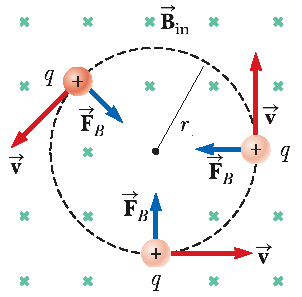
\includegraphics[width=0.4\textwidth]{./thomson_images/Lorentz1.png} 
	\caption{Trajetória circular para uma carga positiva $q$ com velocidade $\vec{v}$ na presença de um campo magnético
    $\vec{B}_{in}$ perpendicular.
    \label{fig:lorentz1}} 
\end{figure}

\begin{figure}[H]
  \centering 
	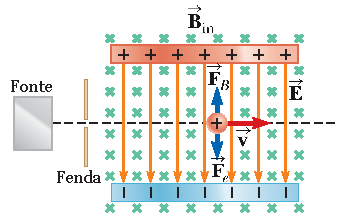
\includegraphics[width=0.5\textwidth]{./thomson_images/Lorentz2.png} 
	\caption{ Carga positiva $q$ com velocidade $\vec{v}$, na presença de um campo magnético $\vec{B}_{in}$ e um campo
    elétrico $\vec{E}$. Os três vetores são mutuamente perpendiculares e estão orientados de modo que as forças têm sentidos
    opostos.
    \label{fig:lorentz2}} 
\end{figure}

\begin{equation}
m\frac{v^2}{R}=qvB \rightarrow R=\frac{mv}{|q|B}
\end{equation}

Um caso particularmente interessante da força de Lorentz verifica-se quando a velocidade da carga é perpendicular tanto
ao campo elétrico como ao magnético. Nesse caso, as duas forças têm a mesma direcção. Adotando uma configuração como a
representada na Fig. \ref{fig:lorentz2}, as forças elétrica e magnética têm sentidos opostos e podem compensar-se,
anulando-se, o que permite que a carga mantenha uma trajetória retilínea.

Nesta repetição da experiência de Thomson iremos utilizar estes dois princípios para determinar a razão $q/m$. Num primeiro
conjunto de medidas, iremos determinar o raio da trajetória de um feixe de raios catódicos na presença de um campo magnético.
No segundo conjunto de medidas iremos equilibrar as forças de um campo magnético e um elétrico de modo a que o feixe tenha
uma forma aproximadamente retilínea.

\newpage
\section{\sf Figuras dos aparelhos da montagem experimental}
\begin{figure}[H]
	\centering 
	\includegraphics[width=0.45\textwidth]{./thomson_images/fig3-ThomsomEquip}
	\caption{Montagem da Experiência de Thomson com tubo de raios catódicos, suporte e par de bobinas de Helmholtz.
    \label{fig:Thomson_Equip}} 
\end{figure}

\begin{figure}[H]
	\centering 
	\includegraphics[width=0.4\textwidth]{./thomson_images/fig4-Thomson_Electron-Deflection-Tube-D}
	\caption{Trajetória dos eletrões sujeitos a um campo magnético perpendicular. \label{fig:Thomson_trajec}} 
\end{figure}



\newpage

\section{\sf Procedimento Experimental}
\subsection {\sf Material}
\begin{enumerate}
	\item Ampola (tubo) de raios catódicos (TRC), modelo TEL 525.
	\item 	Fonte de alimentação do TRC, que inclui alimentação de alta tensão contínua 
	(até 5000 V) aplicada aos elétrodos (cátodo e ânodo) do TRC e alimentação de baixa tensão
	(6.3 V AC) para o filamento do TRC.
	\item Par de bobinas que envolvem a parte esférica do TRC na configuração de
	Helmholtz (para criar um campo magnético aproximadamente homogéneo na
	região central entre as bobinas, de raio médio $r$, e afastadas de $r$ uma da outra).
	\item Fonte de alimentação de corrente \textbf{contínua} (em modo DC) para as bobinas.
	\item Multímetro (como amperímetro) a instalar em \textbf{série} no circuito das bobinas.
\end{enumerate}

O tubo TRC tem um filamento alimentado por 6.3 V (em modo AC). Este filamento emite eletrões por efeito termiónico. 
Entre o ânodo e o cátodo do tubo estabelecem-se diferenças de potencial $ (V_+ - V_-) = U_a$ . Os eletrões são acelerados entre o cátodo e o ânodo e a sua velocidade à saída do ânodo é função de $U_a$. 

Ao entrarem na parte esférica do tubo, os eletrões podem ser defletidos por \emph{campos magnéticos} provocados por
correntes que percorrem as bobinas de Helmholtz e/ou por \emph{campos elétricos} devidos à aplicação de tensão entre
duas placas paralelas ligadas aos pontos 1 e 2 do diagrama (Fig. \ref{fig:TL}).

O campo de indução magnética $B$ devido às bobinas de Helmholtz é aproximadamente uniforme na região central entre as
bobinas, e para uma corrente $I$ é dado por\footnote{No sistema SI, a unidade de campo magnético é o Tesla (T), sendo
1\,T=1\,Weber/m$^{2}$ .}:
\begin{align}
	\label{eq:helmotz}
	 n &= 320\textrm{ espiras} \nonumber \\ 
B = \left(\frac{4}{5}\right)^{3/2} \cdot \frac{\mu_0 n I}{r} =  \frac{32 \pi n }{5 \sqrt{5}} \cdot \frac{I}{r} \cdot 10^{-7}\textrm{ Weber/m}^{2}
 \qquad  r  &= 0.068\textrm{ m} \\
r  &= d/2 \nonumber
\end{align}

\begin{figure}[H]
	[h]  \centering 
	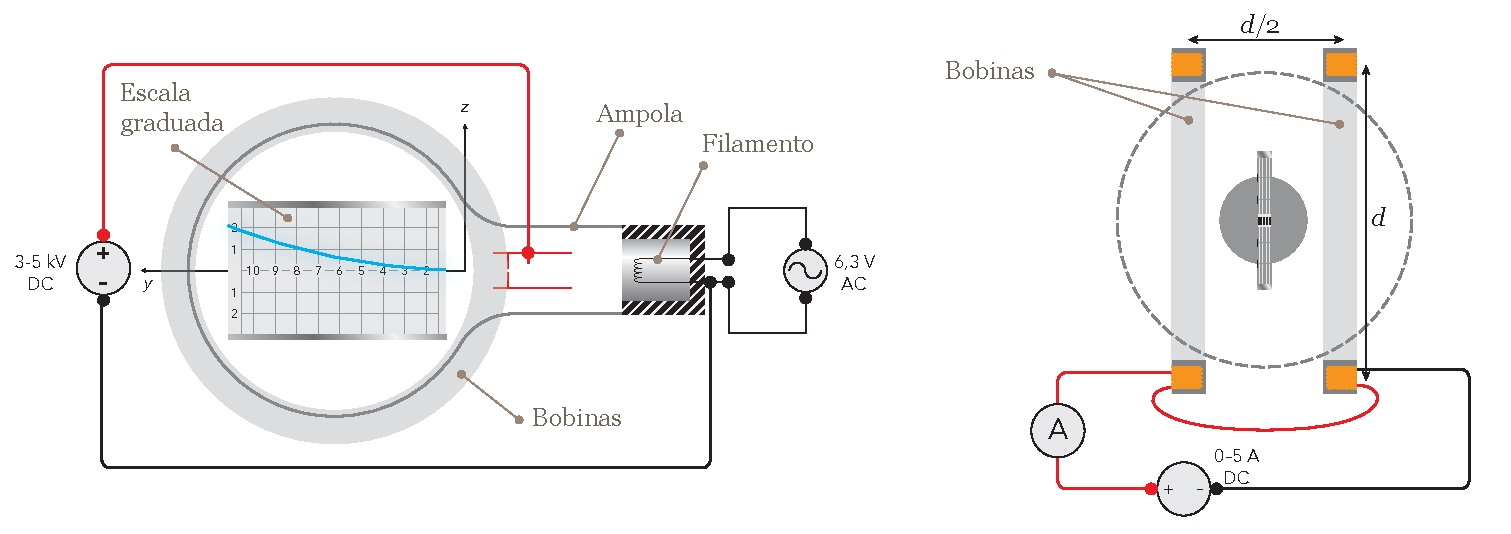
\includegraphics[width=1\textwidth]{thomson_images/fig5-TuboTL.png} 
	\caption{Diagrama do tubo utilizado e geometria das bobinas de Helmholtz. Esquerda: vista lateral, com ligações
    elétricas do filamento e da tensão de aceleração. Direita: vista frontal, com ligações das bobinas de Helmholtz. \label{fig:TL}} 
\end{figure}

\subsection{\sf Determinação de $q/m$ por deflexão magnética}
\subsubsection{\sf Trajetórias de partículas carregadas sujeitas a um campo magnético constante}
Quando se aplica uma tensão $U_a$ entre o ânodo e o cátodo (sem aplicar tensão entre os pontos 1 e 2 representados na Fig.
\ref{fig:TL}), pode admitir-se que a velocidade final $v$ dos eletrões ao abandonarem o ânodo é dada pela seguinte expressão 

\begin{equation}
	\label{eq:encin11}
q\, U_a = \frac{1}{2} m \, v^2
\end{equation}
em que $q$  é a carga do eletrão e $m$ a sua massa.

Os eletrões entram, com velocidade horizontal, na parte esférica do tubo, onde são defletidos pelo campo magnético
$\vec{B}$ (com $\vec{B}\perp\vec{v})$. A sua trajetória passa então a ser circular, com raio $R$, verificando-se:
\begin{equation}
	\label{eq:encin12}
B \, q\, v = \frac{m\,v^2}{R} 
\end{equation}
As trajetórias dos eletrões podem ser visualizadas numa escala graduada feita de material fluorescente. 
A origem do reticulado está situada aproximadamente no início da zona 
sujeita ao campo $\vec{B}$.
Combinando (\ref{eq:encin11}) e (\ref{eq:encin12}) obtém-se uma expressão para a relação $q/m$:
\begin{equation}
	\label{eq:encin3}
 \frac{q}{m} = \frac{2\, U_a}{B^2\,R^2} 
\end{equation}
em que:
\begin{description}
\item[$U_a$] – impõe-se e mede-se diretamente no voltímetro da fonte de tensão.
\item[$B$] – calcula-se, para uma dada corrente $I$, a partir da expressão (\ref{eq:helmotz}).
\item[$R$] – determina-se por leitura no écran fluorescente, das coordenadas de posição $y$ (horizontal) e $z$ (vertical)
de pontos do feixe. Por construção do tubo verifica-se:
\begin{equation}
	\label{eq:eR}
 R = \frac{y^2 + z^2}{2 \, z} 
\end{equation}
\end{description}



\subsubsection{\sf Modo de proceder}


\begin{enumerate}
	\item Montar os circuitos elétricos de acordo com a  Fig. \ref{fig:TL}. Note que as ligações das bobinas devem garantir
    que a corrente elétrica é percorrida no mesmo sentido, em ambas: para isso, deve usar os conetores na ordem
    $A\rightarrow Z$ numa bobina e na ordem inversa na outra bobina. Chamar o docente para verificação, \textbf{antes de ligar os aparelhos}.
	\item Verfifique qual é o valor máximo da tensão disponível na fonte de alta tensão. Escolha um valor ligeiramente inferior.
	\item Ajustar a corrente das bobinas de Helmholtz $I_+$ de modo a que a circunferência passe por um ponto bem
    determinado\footnote{Utilize de preferência os maiores valores possíveis para o raio $R$, de forma a que o feixe
    se encontre na zona central entre as bobines.}.  Calcule $R$.
	Inverta o sentido da corrente e determine um novo $I_-$ para o mesmo raio $R$.
	Tomando $I_{\textrm{medio}} = (I_+ + I_-)/2 $ calcule o campo magnético $B_{\textrm{medio}}$. Utilize a semi-diferença,
     $(I_+ - I_-)/2$, para a estimativa das incertezas $\delta I_{\textrm{medio}}$ e $\delta B_{\textrm{medio}}$.
	\item Repita o ponto 2) para quatro novos valores de $R$. 
	\item Repetir 1), 2) e 3)  e para os mesmos $R$, para dois valores inferiores de tensão, afastados por exemplo de 500 V entre si.
	\item Apresente os valores de $q/m$ para os 15 pares de determinações. Calcule a média desses valores, assim como a incerteza da média.
	\item Para um dos pares de pontos, estime a contribuição relativa das incertezas das grandezas que mediu para a incerteza total. Compare este erro assim calculado com a incerteza calculada a partir dos 15 valores calculados.
	Apresente para cada raio o valor de $q/m$ assim como o erro associado a cada uma das determinações. Compare e comente os resultados.
	\item Apresente um valor final para $q/m$. Estime a precisão e a exatidão obtida nas determinações que realizou.
\end{enumerate}
 
\subsection{\sf Determinação de $q/m$ por deflexão magnética e elétrica quase compensada }

\subsubsection{\sf Situação de equilíbrio entre as interacções elétrica e magnética}

Se, na força de Lorentz, os dois termos se equilibrarem -- ou seja, se as forças eletrostática e magnética forem de igual
módulo e de sentidos opostos -- a carga $q$ não é desviada da sua trajetória. No nosso caso, em que $\vec{B} \perp \vec{v}$,
a condição de equilíbrio é dada por:
\begin{equation}
	\label{eq:equil1}
 |\vec{E}| = v\, |\vec{B}|
\end{equation}

\subsubsection{\sf Montagem a efetuar}

Aproveitando a montagem já efetuada no ponto anterior, ligue agora os terminais 1 e 2 (Fig. \ref{fig:TLE}) à fonte de alta
tensão que gera a tensão $U_a$, produzindo assim na região do écran fluorescente um campo elétrico. Fazendo com que as
bobinas sejam percorridas por uma corrente com intensidade e  ``sentido'' convenientes, podemos obter uma força de origem
magnética anti-paralela à provocada pelo campo $\vec{E}$. 
Deste modo, a trajetória visualizada no écran será aproximadamente retilínea, sendo a condição de equilíbrio dada por:

\begin{equation}
	\label{eq:equil2}
 |\vec{E}| = v\, |\vec{B}| = \frac{U_a}{d}
\end{equation}
onde $d$ é a distância entre as placas do écran fluorescente e $U_a$ a tensão entre as mesmas, que é como se disse igual
à tensão de aceleração.

\begin{figure}[H]
	[h]  \centering 
	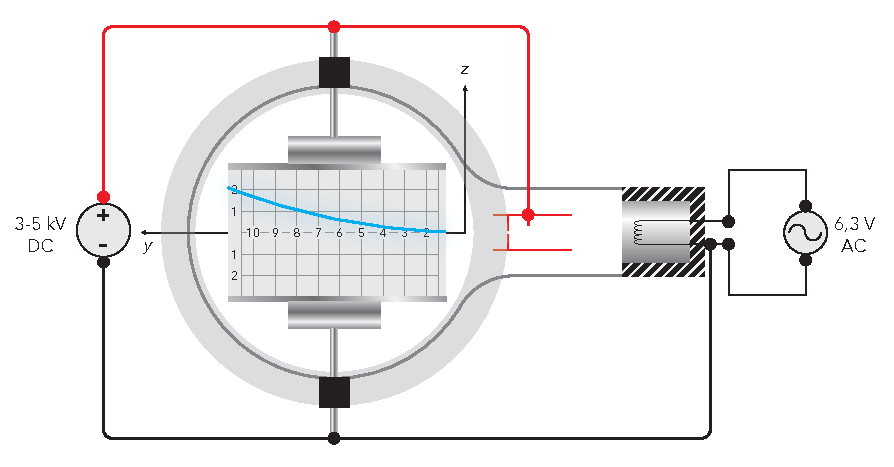
\includegraphics[width=1\textwidth]{thomson_images/fig6-TuboTLE.pdf} 
	\caption{Deflexão magnética e elétrica quase compensada: ligações elétricas do filamento, da tensão de aceleração e
    das placas. \label{fig:TLE}} 
\end{figure}


A equação (\ref{eq:equil2}) permite-nos calcular a velocidade dos eletrões, uma vez que podemos conhecer os valores de
todas as outras variáveis aí intervenientes. O conhecimento de $v$ permite-nos calcular $q/m$ tendo em conta que, segundo
(\ref{eq:encin11}), deverá ser:

\begin{equation*}
\label{eq:encin1}
\frac{q}{m} = \frac{v^2}{2} \; \frac{1}{U_a}
\end{equation*}

Ou finalmente, por combinação com (\ref{eq:equil2}):
\begin{equation}
	\label{eq:qmquase}
\frac{q}{m} = \frac{1}{2} \; \frac{U_a}{B^2\; d^2} 
\end{equation}

\subsubsection{\sf Modo de proceder}
\begin{enumerate}
	\item Para cada uma das quatro tensões de trabalho $U_a$ já referidas, aplicadas agora também às placas que produzem
    o campo elétrico, determine o valor de $B$ (a partir de $I$) que conduz ao anulamento das forças de origem elétrica
    e magnética.
	\item Inverta o sentido dos campos elétricos e magnéticos e repita a determinação do valor de $B$.
	\item Apresente os valores de $q/m$. Analise as diferentes contribuições para a incerteza total. Estime o valor da
    relação carga/massa do eletrão, assim como a precisão e a exatidão obtida nas determinações que realizou.
	\item  Observe  a  trajetória  quando  as  forças  de 
origem elétrica e magnética não se compensam. Comente. 
%	Apresente os valores de q/m calculados assim como o erro associado a cada determinação. Apresente um valor final para $q/m$.
\end{enumerate}

\newpage

\end{document}